\chapter{Proverb 21}
\begin{figure}
  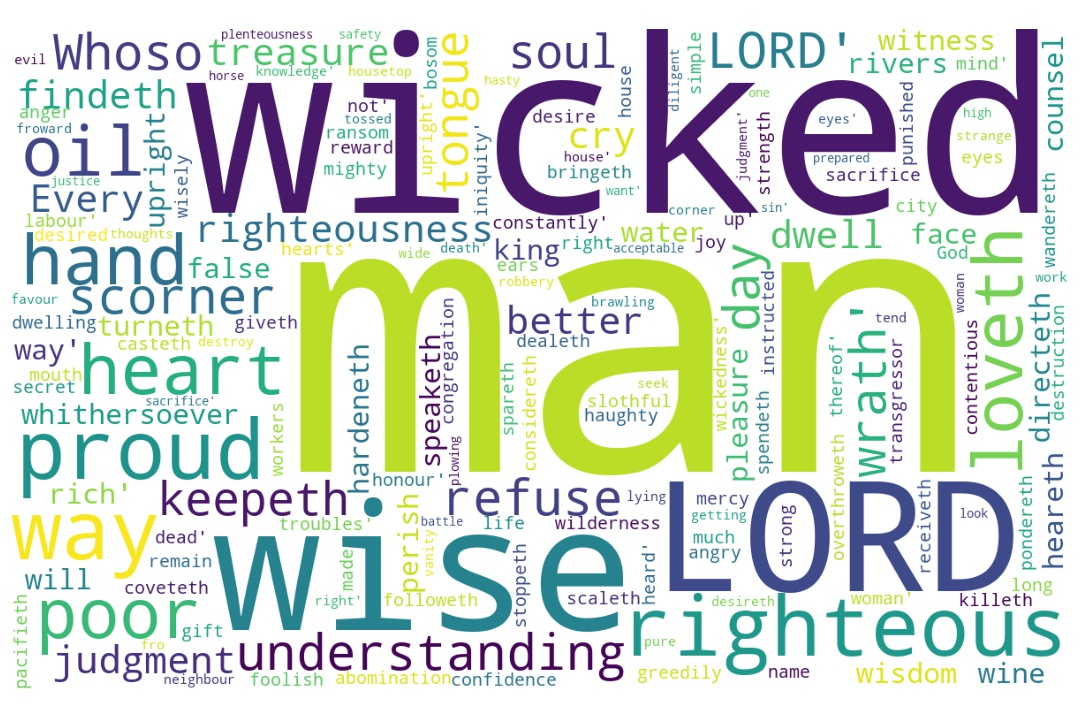
\includegraphics[width=\linewidth]{20OT-Proverbs/Proverb21-WordCloud.jpg}
  \caption{Proverb 21 Word Cloud}
  \label{fig:Proverb 21 word Cloud}
\end{figure}

\marginpar{\scriptsize \centering \fcolorbox{bone}{lime}{\textbf{GOD IN CONTROL OF ALL}}\\ (Proverb 21:1-31) \begin{compactenum}[I.][8]
    \item The \textbf{King's Heart} \index[scripture]{Proverbs!Pro 21:01} (Pro 21:1)
    \item The \textbf{Lord's Hand} \index[scripture]{Proverbs!Pro 21:04} (Pro 21:4)
    \item The \textbf{Look that is High} \index[scripture]{Proverbs!Pro 21:04} (Pro 21:4)
    \item \textbf{Lust that is Hasty} \index[scripture]{Proverbs!Pro 21:05} (Pro 21:5)
    \item \textbf{Languish on the Housetop} \index[scripture]{Proverbs!Pro 21:05} (Pro 21:9)
    \item The \textbf{Lament Unheard} \index[scripture]{Proverbs!Pro 21:13} (Pro 21:13)
    \item The \textbf{Life that is Honored} \index[scripture]{Proverbs!Pro 21:21} (Pro 21:21)
\end{compactenum}}


\marginpar{\scriptsize \centering \fcolorbox{bone}{yellow}{\textbf{LIST OF 13}}\\ (Proverb 21:1-31) \begin{compactenum}[I.][13]
    \item A \textbf{Man} \index[scripture]{Proverbs!Pro 21:02} (Proverbs 21:2)
    \item A \textbf{Proud Heart} \index[scripture]{Proverbs!Pro 21:04} (Proverbs 21:4)
    \item A \textbf{Lying Tongue} \index[scripture]{Proverbs!Pro 21:06} (Proverbs 21:6)
    \item A \textbf{Vanity} \index[scripture]{Proverbs!Pro 21:06} (Proverbs 21:6)
    \item A \textbf{Corner of a House} \index[scripture]{Proverbs!Pro 21:09} (Proverbs 21:9)
    \item A \textbf{Brawling Woman} \index[scripture]{Proverbs!Pro 21:09} (Proverbs 21:9)
    \item A \textbf{Wide House} \index[scripture]{Proverbs!Pro 21:09} (Proverbs 21:9)
    \item A \textbf{Gift} \index[scripture]{Proverbs!Pro 21:14} (Proverbs 21:14)
    \item A \textbf{Poor man} \index[scripture]{Proverbs!Pro 21:17} (Proverbs 21:17)
    \item A \textbf{Ransom} \index[scripture]{Proverbs!Pro 21:18} (Proverbs 21:18)
    \item A \textbf{Contentious and angry woman} \index[scripture]{Proverbs!Pro 21:19} (Proverbs 21:19)
    \item A \textbf{Foolish Man} \index[scripture]{Proverbs!Pro 21:20} (Proverbs 21:20)
    \item A \textbf{Wicked Mind} \index[scripture]{Proverbs!Pro 21:27} (Proverbs 21:27)
\end{compactenum} }

\footnote{\textcolor[cmyk]{0.99998,1,0,0}{\hyperlink{TOC}{Return to end of Table of Contents.}}}\footnote{\href{https://audiobible.com/bible/proverbs_21.html}{\textcolor[cmyk]{0.99998,1,0,0}{Proverbs Audio}}}\textcolor[cmyk]{0.99998,1,0,0}{The \fcolorbox{bone}{lime}{king's heart} \emph{is} in the hand of the LORD, \emph{as} the rivers of water: he turneth it \fcolorbox{bone}{MYGOLD}{whithersoever} he will.}\footnote{\textbf{2 Samuel 14:1} - Now Joab the son of Zeruiah perceived that the king’s heart was toward Absalom.}\footnote{\textbf{Ezra 7:27} - Blessed be the LORD God of our fathers, which hath put such a thing as this in the king’s heart, to beautify the house of the LORD which is in Jerusalem:}
[2] \textcolor[cmyk]{0.99998,1,0,0}{Every way of \fcolorbox{bone}{bone}{a}  man \emph{is} right in his own eyes: but the LORD pondereth the hearts.}\footnote{\textbf{Deuteronomy 12:8} - Ye shall not do after all the things that we do here this day, every man whatsoever is right in his own eyes.}\footnote{\textbF{Judges 17:6} - In those days there was no king in Israel, but every man did that which was right in his own eyes.}\footnote{\textbf{Judges 21:25} - In those days there was no king in Israel: every man did that which was right in his own eyes.}\footnote{\textbf{Proverb 12:15} - The way of a fool is right in his own eyes: but he that hearkeneth unto counsel is wise.}
[3] \textcolor[cmyk]{0.99998,1,0,0}{To do justice and judgment \emph{is} more acceptable to the LORD than sacrifice.}
[4] \textcolor[cmyk]{0.99998,1,0,0}{An \fcolorbox{bone}{lime}{high look}, and \fcolorbox{bone}{bone}{a}  proud heart, \emph{and} the plowing of the wicked, \emph{is} sin.}
[5] \textcolor[cmyk]{0.99998,1,0,0}{The thoughts of the diligent \emph{tend} only to \fcolorbox{bone}{MYGOLD}{plenteousness}; but of every one \emph{that} \emph{is} \fcolorbox{bone}{lime}{hasty only to want}.}
[6] \textcolor[cmyk]{0.99998,1,0,0}{The getting of treasures by \fcolorbox{bone}{bone}{a}  lying tongue \emph{is} \fcolorbox{bone}{bone}{a}  vanity tossed to and fro of them that seek death.}
[7] \textcolor[cmyk]{0.99998,1,0,0}{The robbery of the wicked shall destroy them; because they refuse to do judgment.}
[8] \textcolor[cmyk]{0.99998,1,0,0}{The way of man \emph{is} froward and strange: but \emph{as} \emph{for} the pure, his work \emph{is} right.}
[9] \textcolor[cmyk]{0.99998,1,0,0}{\emph{It} \emph{is} better to dwell in \fcolorbox{bone}{bone}{a}  \fcolorbox{bone}{lime}{corner of the housetop}, than with \fcolorbox{bone}{bone}{a}  brawling woman in \fcolorbox{bone}{bone}{a} wide house.}
[10] \textcolor[cmyk]{0.99998,1,0,0}{The soul of the wicked desireth evil: his neighbour findeth no favour in his eyes.}
[11] \textcolor[cmyk]{0.99998,1,0,0}{When the scorner is punished, the simple is made wise: and when the wise is instructed, he receiveth knowledge.}
[12] \textcolor[cmyk]{0.99998,1,0,0}{The righteous \emph{man} wisely considereth the house of the wicked: \emph{but} \emph{God} overthroweth the wicked for \emph{their} wickedness.}
[13] \textcolor[cmyk]{0.99998,1,0,0}{Whoso stoppeth his ears at \fcolorbox{bone}{lime}{the cry of the poor}, he also shall cry himself, but shall not be heard.}
[14] \textcolor[cmyk]{0.99998,1,0,0}{A gift in secret pacifieth anger: and \fcolorbox{bone}{bone}{a} reward in the bosom strong wrath.}
[15] \textcolor[cmyk]{0.99998,1,0,0}{\emph{It} \emph{is} joy to the just to do judgment: but destruction \emph{shall} \emph{be} to the workers of iniquity.}
[16] \textcolor[cmyk]{0.99998,1,0,0}{The man that wandereth out of the way of \fcolorbox{bone}{MYGOLD}{understanding} shall remain in the congregation of the dead.}
[17] \textcolor[cmyk]{0.99998,1,0,0}{He that loveth pleasure \emph{shall} \emph{be} \fcolorbox{bone}{bone}{a} poor man: he that loveth wine and oil shall not be rich.}
[18] \textcolor[cmyk]{0.99998,1,0,0}{The wicked \emph{shall} \emph{be} \fcolorbox{bone}{bone}{a} ransom for the righteous, and the transgressor for the upright.}
[19] \textcolor[cmyk]{0.99998,1,0,0}{\emph{It} \emph{is} better to dwell in the wilderness, than with \fcolorbox{bone}{bone}{a} contentious and an angry woman.}
[20] \textcolor[cmyk]{0.99998,1,0,0}{\emph{There} \emph{is} treasure to be desired and oil in the dwelling of the wise; but \fcolorbox{bone}{bone}{a} foolish man spendeth it up.}
[21] \textcolor[cmyk]{0.99998,1,0,0}{He that followeth after \fcolorbox{bone}{MYGOLD}{righteousness} and mercy findeth life, \fcolorbox{bone}{MYGOLD}{righteousness}, and \fcolorbox{bone}{lime}{honour}.}
[22] \textcolor[cmyk]{0.99998,1,0,0}{A wise \emph{man} scaleth the city of the mighty, and casteth down the strength of the confidence thereof.}
[23] \textcolor[cmyk]{0.99998,1,0,0}{Whoso keepeth his mouth and his tongue keepeth his soul from troubles.}
[24] \textcolor[cmyk]{0.99998,1,0,0}{Proud \emph{and} haughty scorner \emph{is} his name, who dealeth in proud wrath.}
[25] \textcolor[cmyk]{0.99998,1,0,0}{The desire of the slothful killeth him; for his hands refuse to labour.}
[26] \textcolor[cmyk]{0.99998,1,0,0}{He coveteth greedily all the day long: but the righteous giveth and spareth not.}
[27] \textcolor[cmyk]{0.99998,1,0,0}{The sacrifice of the wicked \emph{is} abomination: how much more, \emph{when} he bringeth it with \fcolorbox{bone}{bone}{a} wicked mind?}
[28] \textcolor[cmyk]{0.99998,1,0,0}{A false witness shall perish: but the man that heareth speaketh constantly.}
[29] \textcolor[cmyk]{0.99998,1,0,0}{A wicked man hardeneth his face: but \emph{as} \emph{for} the upright, he directeth his way.}
[30] \textcolor[cmyk]{0.99998,1,0,0}{\emph{There} \emph{is} no wisdom nor \fcolorbox{bone}{MYGOLD}{understanding} nor counsel against the LORD.}
[31] \textcolor[cmyk]{0.99998,1,0,0}{The horse \emph{is} prepared against the day of battle: but safety \emph{is} of the LORD.}



